
划分树是一种来解决区间第 $K$ 大的一种数据结构, 其常数、理解难度都要比主席树低很多。同时, 划分树紧贴 “第 $K$ 大”,所以是一种基于排序的一种数据结构。

\textbf{建议先学完主席树再看划分树哦}

\subsection{建树}

划分树的建树比较简单, 但是相对于其他树来说比较复杂。

\begin{figure}[htbp]
\centering
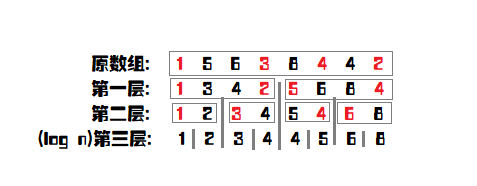
\includegraphics[width=0.7\textwidth]{docs/ds/images/dividing1.png} 

\end{figure}

如图, 每一层都有一个看似无序的数组。其实, 每一个被红色标记的数字都是\textbf{要分配到左儿子的}。而分配的规则是什么? 就是与\textbf{这一层的中位数}做比较, $\leq$ 左边, 否则右边。但是这里要注意一下: 并不是严格的 $\leq$ \textbf{左边, 否则右边}。因为中位数可能有相同, 而且与 $N$ 的奇偶有一定关系。下面的代码展示会有一个巧妙的运用, 大家可以参照代码。

我们不肯能每一次都对每一层排序, 这样子不说常数, 就算是理论复杂度也过不去。我们想, 找中位数, 一次排序就够了。为什么? 比如, 我们求 $l,r$ 的中位数, 其实就是在排完序过后的 $num[mid]$。

两个关键数组:

\begin{minted}{text}
tree[log(N),N]   : 也就是树,要存下所有的值,空间复杂度 $O(n\log n)$。
toleft[log(N),n] : 也就是每一层 1~i 进入左儿子的数量,这里需要理解一下,这是一个前缀和。
\end{minted}

\begin{minted}{pascal}
procedure Build(left,right,deep:longint); // left,right 是左右区间,deep是第几层
var
  i,mid,same,ls,rs,flag:longint; // 其中 flag 是用来平衡左右两边的数量的
begin
  if left=right then exit; // 到底层了
  mid:=(left+right) >> 1;
  same:=mid-left+1;
  for i:=left to right do 
    if tree[deep,i]<num[mid] then
      dec(same);

  ls:=left; // 分配到左儿子的第一个指针
  rs:=mid+1; // 分配到右儿子的第一个指针
  for i:=left to right do
  begin
    flag:=0;
    if (tree[deep,i]<num[mid])or((tree[deep,i]=num[mid])and(same>0)) then // 分配到左边的条件
    begin
      flag:=1; tree[deep+1,ls]:=tree[deep,i]; inc(ls);
      if tree[deep,i]=num[mid] then // 平衡左右个数
        dec(same);
    end
    else
    begin
      tree[deep+1,rs]:=tree[deep,i]; inc(rs);
    end;
    toleft[deep,i]:=toleft[deep,i-1]+flag;
  end;
  Build(left,mid,deep+1); // 继续
  Build(mid+1,right,deep+1);
end;
\end{minted}

\subsection{查询}

那我们先扯一下主席树的内容。在用主席树求区间第 $K$ 小的时候, 我们以 $K$ 为基准, 向左就向左, 向右要减去向左的值, 在划分树中也是这样子的。

查询难理解的, 在于 \textbf{区间缩小} 这种东西。下图, 我查询的是 $3$ 到 $7$, 那么下一层我就只需要查询 $2$ 到 $3$ 了。当然, 我们定义 $left,right$ 为缩小后的区间 (目标区间), $l,r$ 还是我所在节点的区间。那为什么要标出目标区间呢? 因为那是\textbf{判定答案在左边, 右边的基准}。

 \begin{figure}[htbp]
\centering
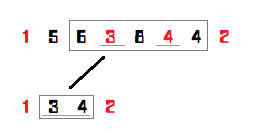
\includegraphics[width=0.7\textwidth]{docs/ds/images/dividing2.png} 

\end{figure}

\begin{minted}{pascal}
function Query(left,right,k,l,r,deep:longint):longint;
var
  mid,x,y,cnt,rx,ry:longint;
begin
  if left=right then // 写成 l=r 也无妨,因为目标区间也一定有答案
    exit(tree[deep,left]);
  mid:=(l+r) >> 1;
  x:=toleft[deep,left-1]-toleft[deep,l-1]; // l 到 left 的去左儿子的个数
  y:=toleft[deep,right]-toleft[deep,l-1]; // l 到 right 的去左儿子的个数
  ry:=right-l-y; rx:=left-l-x; // ry 是 l 到 right 去右儿子的个数,rx 则是 l 到 lefr 去右儿子的个数
  cnt:=y-x; // left 到 right 左儿子的个数
  if cnt>=k then // 主席树常识啦
    Query:=Query(l+x,l+y-1,k,l,mid,deep+1) // l+x 就是缩小左边界,l+y-1 就是缩小右区间。对于上图来说,就是把 1 和 2 放弃了。
  else
    Query:=Query(mid+rx+1,mid+ry+1,k-cnt,mid+1,r,deep+1); // 同样是缩小区间,只不过变成了右边而已。注意要 k-cnt。
end;
\end{minted}

\subsection{理论复杂度和亲测结果}

时间复杂度 : 一次查询只需要 $O(\log n)$,$m$次询问, 就是 $O(m\log n)$。

空间复杂度 : 只需要存储 $O(n\log n)$ 个数字。

亲测结果:  主席树 : $1482 \text{ms}$、划分树 : $889 \text{ms}$。 (非递归, 常数比较小)

\subsection{后记}

大家可以试着去写非递归版哦。参考博文 : \href{https://blog.csdn.net/littlewhite520/article/details/70250722}{传送门}。
